% Created by tikzDevice version 0.12 on 2019-04-08 12:48:38
% !TEX encoding = UTF-8 Unicode
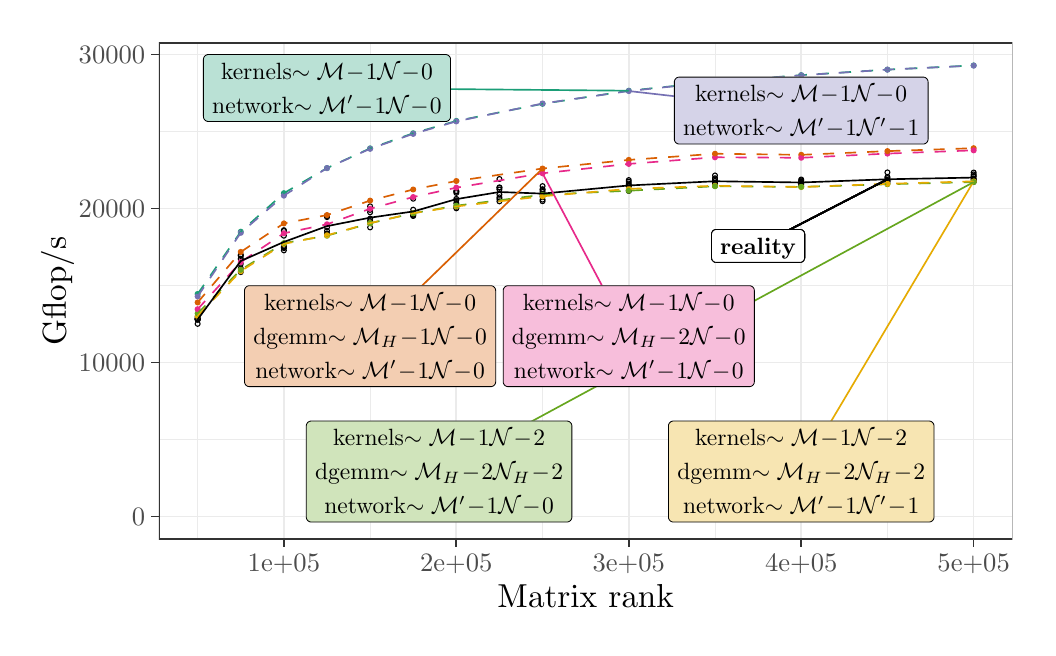
\begin{tikzpicture}[x=1pt,y=1pt]
\definecolor{fillColor}{RGB}{255,255,255}
\path[use as bounding box,fill=fillColor,fill opacity=0.00] (0,0) rectangle (361.35,216.81);
\begin{scope}
\path[clip] (  0.00,  0.00) rectangle (361.35,216.81);
\definecolor{drawColor}{RGB}{255,255,255}
\definecolor{fillColor}{RGB}{255,255,255}

\path[draw=drawColor,line width= 0.6pt,line join=round,line cap=round,fill=fillColor] (  0.00,  0.00) rectangle (361.35,216.81);
\end{scope}
\begin{scope}
\path[clip] ( 47.40, 31.96) rectangle (355.85,211.31);
\definecolor{fillColor}{RGB}{255,255,255}

\path[fill=fillColor] ( 47.40, 31.96) rectangle (355.85,211.31);
\definecolor{drawColor}{gray}{0.92}

\path[draw=drawColor,line width= 0.3pt,line join=round] ( 47.40, 67.96) --
	(355.85, 67.96);

\path[draw=drawColor,line width= 0.3pt,line join=round] ( 47.40,123.64) --
	(355.85,123.64);

\path[draw=drawColor,line width= 0.3pt,line join=round] ( 47.40,179.33) --
	(355.85,179.33);

\path[draw=drawColor,line width= 0.3pt,line join=round] ( 61.42, 31.96) --
	( 61.42,211.31);

\path[draw=drawColor,line width= 0.3pt,line join=round] (123.74, 31.96) --
	(123.74,211.31);

\path[draw=drawColor,line width= 0.3pt,line join=round] (186.05, 31.96) --
	(186.05,211.31);

\path[draw=drawColor,line width= 0.3pt,line join=round] (248.36, 31.96) --
	(248.36,211.31);

\path[draw=drawColor,line width= 0.3pt,line join=round] (310.67, 31.96) --
	(310.67,211.31);

\path[draw=drawColor,line width= 0.6pt,line join=round] ( 47.40, 40.12) --
	(355.85, 40.12);

\path[draw=drawColor,line width= 0.6pt,line join=round] ( 47.40, 95.80) --
	(355.85, 95.80);

\path[draw=drawColor,line width= 0.6pt,line join=round] ( 47.40,151.48) --
	(355.85,151.48);

\path[draw=drawColor,line width= 0.6pt,line join=round] ( 47.40,207.17) --
	(355.85,207.17);

\path[draw=drawColor,line width= 0.6pt,line join=round] ( 92.58, 31.96) --
	( 92.58,211.31);

\path[draw=drawColor,line width= 0.6pt,line join=round] (154.89, 31.96) --
	(154.89,211.31);

\path[draw=drawColor,line width= 0.6pt,line join=round] (217.20, 31.96) --
	(217.20,211.31);

\path[draw=drawColor,line width= 0.6pt,line join=round] (279.52, 31.96) --
	(279.52,211.31);

\path[draw=drawColor,line width= 0.6pt,line join=round] (341.83, 31.96) --
	(341.83,211.31);
\definecolor{drawColor}{RGB}{0,0,0}

\path[draw=drawColor,line width= 0.4pt,line join=round,line cap=round] (341.83,164.46) circle (  0.89);

\path[draw=drawColor,line width= 0.4pt,line join=round,line cap=round] ( 61.42,111.28) circle (  0.89);

\path[draw=drawColor,line width= 0.4pt,line join=round,line cap=round] (217.20,157.83) circle (  0.89);

\path[draw=drawColor,line width= 0.4pt,line join=round,line cap=round] (279.52,160.73) circle (  0.89);

\path[draw=drawColor,line width= 0.4pt,line join=round,line cap=round] (123.74,150.98) circle (  0.89);

\path[draw=drawColor,line width= 0.4pt,line join=round,line cap=round] (186.05,154.66) circle (  0.89);

\path[draw=drawColor,line width= 0.4pt,line join=round,line cap=round] (310.67,162.84) circle (  0.89);

\path[draw=drawColor,line width= 0.4pt,line join=round,line cap=round] (248.36,163.40) circle (  0.89);

\path[draw=drawColor,line width= 0.4pt,line join=round,line cap=round] (154.89,154.94) circle (  0.89);

\path[draw=drawColor,line width= 0.4pt,line join=round,line cap=round] ( 92.58,143.35) circle (  0.89);

\path[draw=drawColor,line width= 0.4pt,line join=round,line cap=round] ( 77.00,134.72) circle (  0.89);

\path[draw=drawColor,line width= 0.4pt,line join=round,line cap=round] (108.16,148.37) circle (  0.89);

\path[draw=drawColor,line width= 0.4pt,line join=round,line cap=round] (170.47,159.11) circle (  0.89);

\path[draw=drawColor,line width= 0.4pt,line join=round,line cap=round] ( 77.00,134.56) circle (  0.89);

\path[draw=drawColor,line width= 0.4pt,line join=round,line cap=round] (217.20,161.73) circle (  0.89);

\path[draw=drawColor,line width= 0.4pt,line join=round,line cap=round] (310.67,164.51) circle (  0.89);

\path[draw=drawColor,line width= 0.4pt,line join=round,line cap=round] (154.89,157.78) circle (  0.89);

\path[draw=drawColor,line width= 0.4pt,line join=round,line cap=round] (139.31,148.92) circle (  0.89);

\path[draw=drawColor,line width= 0.4pt,line join=round,line cap=round] ( 61.42,111.34) circle (  0.89);

\path[draw=drawColor,line width= 0.4pt,line join=round,line cap=round] (170.47,162.12) circle (  0.89);

\path[draw=drawColor,line width= 0.4pt,line join=round,line cap=round] (186.05,158.44) circle (  0.89);

\path[draw=drawColor,line width= 0.4pt,line join=round,line cap=round] (108.16,142.13) circle (  0.89);

\path[draw=drawColor,line width= 0.4pt,line join=round,line cap=round] (123.74,147.81) circle (  0.89);

\path[draw=drawColor,line width= 0.4pt,line join=round,line cap=round] ( 92.58,143.63) circle (  0.89);

\path[draw=drawColor,line width= 0.4pt,line join=round,line cap=round] (341.83,163.23) circle (  0.89);

\path[draw=drawColor,line width= 0.4pt,line join=round,line cap=round] (279.52,161.95) circle (  0.89);

\path[draw=drawColor,line width= 0.4pt,line join=round,line cap=round] (248.36,159.89) circle (  0.89);

\path[draw=drawColor,line width= 0.4pt,line join=round,line cap=round] ( 61.42,111.61) circle (  0.89);

\path[draw=drawColor,line width= 0.4pt,line join=round,line cap=round] (108.16,141.96) circle (  0.89);

\path[draw=drawColor,line width= 0.4pt,line join=round,line cap=round] (341.83,161.40) circle (  0.89);

\path[draw=drawColor,line width= 0.4pt,line join=round,line cap=round] (170.47,154.88) circle (  0.89);

\path[draw=drawColor,line width= 0.4pt,line join=round,line cap=round] (123.74,150.09) circle (  0.89);

\path[draw=drawColor,line width= 0.4pt,line join=round,line cap=round] (279.52,161.17) circle (  0.89);

\path[draw=drawColor,line width= 0.4pt,line join=round,line cap=round] ( 77.00,129.88) circle (  0.89);

\path[draw=drawColor,line width= 0.4pt,line join=round,line cap=round] (217.20,159.61) circle (  0.89);

\path[draw=drawColor,line width= 0.4pt,line join=round,line cap=round] (248.36,161.45) circle (  0.89);

\path[draw=drawColor,line width= 0.4pt,line join=round,line cap=round] (310.67,162.45) circle (  0.89);

\path[draw=drawColor,line width= 0.4pt,line join=round,line cap=round] (186.05,155.77) circle (  0.89);

\path[draw=drawColor,line width= 0.4pt,line join=round,line cap=round] (154.89,157.11) circle (  0.89);

\path[draw=drawColor,line width= 0.4pt,line join=round,line cap=round] ( 92.58,137.17) circle (  0.89);

\path[draw=drawColor,line width= 0.4pt,line join=round,line cap=round] (139.31,149.20) circle (  0.89);

\path[draw=drawColor,line width= 0.4pt,line join=round,line cap=round] (186.05,157.50) circle (  0.89);

\path[draw=drawColor,line width= 0.4pt,line join=round,line cap=round] ( 61.42,109.78) circle (  0.89);

\path[draw=drawColor,line width= 0.4pt,line join=round,line cap=round] (217.20,159.56) circle (  0.89);

\path[draw=drawColor,line width= 0.4pt,line join=round,line cap=round] (108.16,142.46) circle (  0.89);

\path[draw=drawColor,line width= 0.4pt,line join=round,line cap=round] ( 92.58,137.90) circle (  0.89);

\path[draw=drawColor,line width= 0.4pt,line join=round,line cap=round] (341.83,163.79) circle (  0.89);

\path[draw=drawColor,line width= 0.4pt,line join=round,line cap=round] ( 77.00,133.33) circle (  0.89);

\path[draw=drawColor,line width= 0.4pt,line join=round,line cap=round] (123.74,146.42) circle (  0.89);

\path[draw=drawColor,line width= 0.4pt,line join=round,line cap=round] (154.89,154.43) circle (  0.89);

\path[draw=drawColor,line width= 0.4pt,line join=round,line cap=round] (279.52,161.17) circle (  0.89);

\path[draw=drawColor,line width= 0.4pt,line join=round,line cap=round] (170.47,156.50) circle (  0.89);

\path[draw=drawColor,line width= 0.4pt,line join=round,line cap=round] (310.67,160.56) circle (  0.89);

\path[draw=drawColor,line width= 0.4pt,line join=round,line cap=round] (139.31,149.42) circle (  0.89);

\path[draw=drawColor,line width= 0.4pt,line join=round,line cap=round] (248.36,160.84) circle (  0.89);

\path[draw=drawColor,line width= 0.4pt,line join=round,line cap=round] (154.89,152.04) circle (  0.89);

\path[draw=drawColor,line width= 0.4pt,line join=round,line cap=round] (310.67,161.40) circle (  0.89);

\path[draw=drawColor,line width= 0.4pt,line join=round,line cap=round] (139.31,151.04) circle (  0.89);

\path[draw=drawColor,line width= 0.4pt,line join=round,line cap=round] (279.52,159.61) circle (  0.89);

\path[draw=drawColor,line width= 0.4pt,line join=round,line cap=round] (186.05,156.61) circle (  0.89);

\path[draw=drawColor,line width= 0.4pt,line join=round,line cap=round] ( 61.42,112.28) circle (  0.89);

\path[draw=drawColor,line width= 0.4pt,line join=round,line cap=round] (217.20,160.00) circle (  0.89);

\path[draw=drawColor,line width= 0.4pt,line join=round,line cap=round] (341.83,161.06) circle (  0.89);

\path[draw=drawColor,line width= 0.4pt,line join=round,line cap=round] ( 77.00,134.33) circle (  0.89);

\path[draw=drawColor,line width= 0.4pt,line join=round,line cap=round] (108.16,148.81) circle (  0.89);

\path[draw=drawColor,line width= 0.4pt,line join=round,line cap=round] (123.74,152.26) circle (  0.89);

\path[draw=drawColor,line width= 0.4pt,line join=round,line cap=round] ( 92.58,136.34) circle (  0.89);

\path[draw=drawColor,line width= 0.4pt,line join=round,line cap=round] (170.47,155.49) circle (  0.89);

\path[draw=drawColor,line width= 0.4pt,line join=round,line cap=round] (248.36,159.72) circle (  0.89);

\path[draw=drawColor,line width= 0.4pt,line join=round,line cap=round] (341.83,161.95) circle (  0.89);

\path[draw=drawColor,line width= 0.4pt,line join=round,line cap=round] ( 61.42,111.39) circle (  0.89);

\path[draw=drawColor,line width= 0.4pt,line join=round,line cap=round] (217.20,157.89) circle (  0.89);

\path[draw=drawColor,line width= 0.4pt,line join=round,line cap=round] (279.52,160.50) circle (  0.89);

\path[draw=drawColor,line width= 0.4pt,line join=round,line cap=round] (123.74,146.92) circle (  0.89);

\path[draw=drawColor,line width= 0.4pt,line join=round,line cap=round] (186.05,158.17) circle (  0.89);

\path[draw=drawColor,line width= 0.4pt,line join=round,line cap=round] (310.67,161.45) circle (  0.89);

\path[draw=drawColor,line width= 0.4pt,line join=round,line cap=round] (248.36,160.73) circle (  0.89);

\path[draw=drawColor,line width= 0.4pt,line join=round,line cap=round] (154.89,151.54) circle (  0.89);

\path[draw=drawColor,line width= 0.4pt,line join=round,line cap=round] ( 92.58,137.45) circle (  0.89);

\path[draw=drawColor,line width= 0.4pt,line join=round,line cap=round] ( 77.00,131.44) circle (  0.89);

\path[draw=drawColor,line width= 0.4pt,line join=round,line cap=round] (108.16,148.87) circle (  0.89);

\path[draw=drawColor,line width= 0.4pt,line join=round,line cap=round] (170.47,158.33) circle (  0.89);

\path[draw=drawColor,line width= 0.4pt,line join=round,line cap=round] ( 77.00,128.49) circle (  0.89);

\path[draw=drawColor,line width= 0.4pt,line join=round,line cap=round] (217.20,161.17) circle (  0.89);

\path[draw=drawColor,line width= 0.4pt,line join=round,line cap=round] (310.67,161.17) circle (  0.89);

\path[draw=drawColor,line width= 0.4pt,line join=round,line cap=round] (154.89,153.38) circle (  0.89);

\path[draw=drawColor,line width= 0.4pt,line join=round,line cap=round] (139.31,154.99) circle (  0.89);

\path[draw=drawColor,line width= 0.4pt,line join=round,line cap=round] ( 61.42,111.61) circle (  0.89);

\path[draw=drawColor,line width= 0.4pt,line join=round,line cap=round] (170.47,154.05) circle (  0.89);

\path[draw=drawColor,line width= 0.4pt,line join=round,line cap=round] (186.05,154.10) circle (  0.89);

\path[draw=drawColor,line width= 0.4pt,line join=round,line cap=round] (108.16,144.69) circle (  0.89);

\path[draw=drawColor,line width= 0.4pt,line join=round,line cap=round] (123.74,144.63) circle (  0.89);

\path[draw=drawColor,line width= 0.4pt,line join=round,line cap=round] ( 92.58,137.56) circle (  0.89);

\path[draw=drawColor,line width= 0.4pt,line join=round,line cap=round] (341.83,162.23) circle (  0.89);

\path[draw=drawColor,line width= 0.4pt,line join=round,line cap=round] (279.52,161.62) circle (  0.89);

\path[draw=drawColor,line width= 0.4pt,line join=round,line cap=round] (248.36,162.06) circle (  0.89);

\path[draw=drawColor,line width= 0.4pt,line join=round,line cap=round] ( 61.42,111.73) circle (  0.89);

\path[draw=drawColor,line width= 0.4pt,line join=round,line cap=round] (108.16,143.41) circle (  0.89);

\path[draw=drawColor,line width= 0.4pt,line join=round,line cap=round] (341.83,163.01) circle (  0.89);

\path[draw=drawColor,line width= 0.4pt,line join=round,line cap=round] (170.47,158.95) circle (  0.89);

\path[draw=drawColor,line width= 0.4pt,line join=round,line cap=round] (123.74,146.19) circle (  0.89);

\path[draw=drawColor,line width= 0.4pt,line join=round,line cap=round] (279.52,160.23) circle (  0.89);

\path[draw=drawColor,line width= 0.4pt,line join=round,line cap=round] ( 77.00,133.16) circle (  0.89);

\path[draw=drawColor,line width= 0.4pt,line join=round,line cap=round] (217.20,160.50) circle (  0.89);

\path[draw=drawColor,line width= 0.4pt,line join=round,line cap=round] (248.36,162.40) circle (  0.89);

\path[draw=drawColor,line width= 0.4pt,line join=round,line cap=round] (310.67,161.84) circle (  0.89);

\path[draw=drawColor,line width= 0.4pt,line join=round,line cap=round] (186.05,159.56) circle (  0.89);

\path[draw=drawColor,line width= 0.4pt,line join=round,line cap=round] (154.89,157.55) circle (  0.89);

\path[draw=drawColor,line width= 0.4pt,line join=round,line cap=round] ( 92.58,141.63) circle (  0.89);

\path[draw=drawColor,line width= 0.4pt,line join=round,line cap=round] (139.31,148.76) circle (  0.89);
\definecolor{drawColor}{RGB}{230,171,2}
\definecolor{fillColor}{RGB}{230,171,2}

\path[draw=drawColor,line width= 0.4pt,line join=round,line cap=round,fill=fillColor] ( 77.00,128.82) circle (  0.89);

\path[draw=drawColor,line width= 0.4pt,line join=round,line cap=round,fill=fillColor] (139.31,149.76) circle (  0.89);

\path[draw=drawColor,line width= 0.4pt,line join=round,line cap=round,fill=fillColor] (248.36,159.67) circle (  0.89);
\definecolor{drawColor}{RGB}{217,95,2}
\definecolor{fillColor}{RGB}{217,95,2}

\path[draw=drawColor,line width= 0.4pt,line join=round,line cap=round,fill=fillColor] ( 61.42,117.52) circle (  0.89);

\path[draw=drawColor,line width= 0.4pt,line join=round,line cap=round,fill=fillColor] (123.74,154.32) circle (  0.89);

\path[draw=drawColor,line width= 0.4pt,line join=round,line cap=round,fill=fillColor] (217.20,169.02) circle (  0.89);

\path[draw=drawColor,line width= 0.4pt,line join=round,line cap=round,fill=fillColor] (341.83,173.26) circle (  0.89);
\definecolor{drawColor}{RGB}{230,171,2}
\definecolor{fillColor}{RGB}{230,171,2}

\path[draw=drawColor,line width= 0.4pt,line join=round,line cap=round,fill=fillColor] ( 92.58,138.68) circle (  0.89);

\path[draw=drawColor,line width= 0.4pt,line join=round,line cap=round,fill=fillColor] (154.89,152.21) circle (  0.89);

\path[draw=drawColor,line width= 0.4pt,line join=round,line cap=round,fill=fillColor] (279.52,159.22) circle (  0.89);

\path[draw=drawColor,line width= 0.4pt,line join=round,line cap=round,fill=fillColor] ( 61.42,112.62) circle (  0.89);

\path[draw=drawColor,line width= 0.4pt,line join=round,line cap=round,fill=fillColor] (123.74,146.19) circle (  0.89);

\path[draw=drawColor,line width= 0.4pt,line join=round,line cap=round,fill=fillColor] (217.20,158.56) circle (  0.89);

\path[draw=drawColor,line width= 0.4pt,line join=round,line cap=round,fill=fillColor] (341.83,161.28) circle (  0.89);
\definecolor{drawColor}{RGB}{231,41,138}
\definecolor{fillColor}{RGB}{231,41,138}

\path[draw=drawColor,line width= 0.4pt,line join=round,line cap=round,fill=fillColor] ( 77.00,132.11) circle (  0.89);

\path[draw=drawColor,line width= 0.4pt,line join=round,line cap=round,fill=fillColor] (139.31,155.60) circle (  0.89);

\path[draw=drawColor,line width= 0.4pt,line join=round,line cap=round,fill=fillColor] (248.36,169.97) circle (  0.89);
\definecolor{drawColor}{RGB}{102,166,30}
\definecolor{fillColor}{RGB}{102,166,30}

\path[draw=drawColor,line width= 0.4pt,line join=round,line cap=round,fill=fillColor] ( 61.42,113.56) circle (  0.89);

\path[draw=drawColor,line width= 0.4pt,line join=round,line cap=round,fill=fillColor] (123.74,146.14) circle (  0.89);

\path[draw=drawColor,line width= 0.4pt,line join=round,line cap=round,fill=fillColor] (217.20,157.89) circle (  0.89);

\path[draw=drawColor,line width= 0.4pt,line join=round,line cap=round,fill=fillColor] (341.83,161.01) circle (  0.89);
\definecolor{drawColor}{RGB}{231,41,138}
\definecolor{fillColor}{RGB}{231,41,138}

\path[draw=drawColor,line width= 0.4pt,line join=round,line cap=round,fill=fillColor] ( 61.42,115.07) circle (  0.89);

\path[draw=drawColor,line width= 0.4pt,line join=round,line cap=round,fill=fillColor] (123.74,151.37) circle (  0.89);

\path[draw=drawColor,line width= 0.4pt,line join=round,line cap=round,fill=fillColor] (217.20,167.58) circle (  0.89);

\path[draw=drawColor,line width= 0.4pt,line join=round,line cap=round,fill=fillColor] (341.83,172.48) circle (  0.89);

\path[draw=drawColor,line width= 0.4pt,line join=round,line cap=round,fill=fillColor] (108.16,145.75) circle (  0.89);

\path[draw=drawColor,line width= 0.4pt,line join=round,line cap=round,fill=fillColor] (186.05,164.18) circle (  0.89);

\path[draw=drawColor,line width= 0.4pt,line join=round,line cap=round,fill=fillColor] (310.67,171.31) circle (  0.89);
\definecolor{drawColor}{RGB}{217,95,2}
\definecolor{fillColor}{RGB}{217,95,2}

\path[draw=drawColor,line width= 0.4pt,line join=round,line cap=round,fill=fillColor] ( 77.00,135.78) circle (  0.89);

\path[draw=drawColor,line width= 0.4pt,line join=round,line cap=round,fill=fillColor] (139.31,158.33) circle (  0.89);

\path[draw=drawColor,line width= 0.4pt,line join=round,line cap=round,fill=fillColor] (248.36,171.25) circle (  0.89);

\path[draw=drawColor,line width= 0.4pt,line join=round,line cap=round,fill=fillColor] (108.16,149.09) circle (  0.89);

\path[draw=drawColor,line width= 0.4pt,line join=round,line cap=round,fill=fillColor] (186.05,165.91) circle (  0.89);

\path[draw=drawColor,line width= 0.4pt,line join=round,line cap=round,fill=fillColor] (310.67,172.20) circle (  0.89);
\definecolor{drawColor}{RGB}{102,166,30}
\definecolor{fillColor}{RGB}{102,166,30}

\path[draw=drawColor,line width= 0.4pt,line join=round,line cap=round,fill=fillColor] (108.16,141.63) circle (  0.89);

\path[draw=drawColor,line width= 0.4pt,line join=round,line cap=round,fill=fillColor] (186.05,156.44) circle (  0.89);

\path[draw=drawColor,line width= 0.4pt,line join=round,line cap=round,fill=fillColor] (310.67,160.23) circle (  0.89);
\definecolor{drawColor}{RGB}{230,171,2}
\definecolor{fillColor}{RGB}{230,171,2}

\path[draw=drawColor,line width= 0.4pt,line join=round,line cap=round,fill=fillColor] (108.16,141.79) circle (  0.89);

\path[draw=drawColor,line width= 0.4pt,line join=round,line cap=round,fill=fillColor] (186.05,155.88) circle (  0.89);

\path[draw=drawColor,line width= 0.4pt,line join=round,line cap=round,fill=fillColor] (310.67,160.39) circle (  0.89);
\definecolor{drawColor}{RGB}{102,166,30}
\definecolor{fillColor}{RGB}{102,166,30}

\path[draw=drawColor,line width= 0.4pt,line join=round,line cap=round,fill=fillColor] ( 77.00,129.32) circle (  0.89);

\path[draw=drawColor,line width= 0.4pt,line join=round,line cap=round,fill=fillColor] (139.31,149.76) circle (  0.89);

\path[draw=drawColor,line width= 0.4pt,line join=round,line cap=round,fill=fillColor] (248.36,159.50) circle (  0.89);

\path[draw=drawColor,line width= 0.4pt,line join=round,line cap=round,fill=fillColor] ( 92.58,138.95) circle (  0.89);

\path[draw=drawColor,line width= 0.4pt,line join=round,line cap=round,fill=fillColor] (154.89,152.49) circle (  0.89);

\path[draw=drawColor,line width= 0.4pt,line join=round,line cap=round,fill=fillColor] (279.52,159.28) circle (  0.89);
\definecolor{drawColor}{RGB}{217,95,2}
\definecolor{fillColor}{RGB}{217,95,2}

\path[draw=drawColor,line width= 0.4pt,line join=round,line cap=round,fill=fillColor] ( 92.58,146.08) circle (  0.89);

\path[draw=drawColor,line width= 0.4pt,line join=round,line cap=round,fill=fillColor] (154.89,161.40) circle (  0.89);

\path[draw=drawColor,line width= 0.4pt,line join=round,line cap=round,fill=fillColor] (279.52,170.86) circle (  0.89);
\definecolor{drawColor}{RGB}{231,41,138}
\definecolor{fillColor}{RGB}{231,41,138}

\path[draw=drawColor,line width= 0.4pt,line join=round,line cap=round,fill=fillColor] ( 92.58,142.52) circle (  0.89);

\path[draw=drawColor,line width= 0.4pt,line join=round,line cap=round,fill=fillColor] (154.89,159.00) circle (  0.89);

\path[draw=drawColor,line width= 0.4pt,line join=round,line cap=round,fill=fillColor] (279.52,169.80) circle (  0.89);
\definecolor{drawColor}{RGB}{27,158,119}
\definecolor{fillColor}{RGB}{27,158,119}

\path[draw=drawColor,line width= 0.4pt,line join=round,line cap=round,fill=fillColor] (341.83,203.16) circle (  0.89);

\path[draw=drawColor,line width= 0.4pt,line join=round,line cap=round,fill=fillColor] ( 61.42,120.58) circle (  0.89);

\path[draw=drawColor,line width= 0.4pt,line join=round,line cap=round,fill=fillColor] (217.20,194.03) circle (  0.89);

\path[draw=drawColor,line width= 0.4pt,line join=round,line cap=round,fill=fillColor] (279.52,199.65) circle (  0.89);

\path[draw=drawColor,line width= 0.4pt,line join=round,line cap=round,fill=fillColor] (123.74,173.20) circle (  0.89);

\path[draw=drawColor,line width= 0.4pt,line join=round,line cap=round,fill=fillColor] (154.89,183.11) circle (  0.89);

\path[draw=drawColor,line width= 0.4pt,line join=round,line cap=round,fill=fillColor] ( 92.58,157.00) circle (  0.89);

\path[draw=drawColor,line width= 0.4pt,line join=round,line cap=round,fill=fillColor] (139.31,178.66) circle (  0.89);

\path[draw=drawColor,line width= 0.4pt,line join=round,line cap=round,fill=fillColor] (186.05,189.29) circle (  0.89);

\path[draw=drawColor,line width= 0.4pt,line join=round,line cap=round,fill=fillColor] (310.67,201.65) circle (  0.89);

\path[draw=drawColor,line width= 0.4pt,line join=round,line cap=round,fill=fillColor] (248.36,197.26) circle (  0.89);

\path[draw=drawColor,line width= 0.4pt,line join=round,line cap=round,fill=fillColor] ( 77.00,143.08) circle (  0.89);

\path[draw=drawColor,line width= 0.4pt,line join=round,line cap=round,fill=fillColor] (108.16,166.07) circle (  0.89);
\definecolor{drawColor}{RGB}{117,112,179}
\definecolor{fillColor}{RGB}{117,112,179}

\path[draw=drawColor,line width= 0.4pt,line join=round,line cap=round,fill=fillColor] (341.83,203.10) circle (  0.89);

\path[draw=drawColor,line width= 0.4pt,line join=round,line cap=round,fill=fillColor] ( 61.42,119.69) circle (  0.89);

\path[draw=drawColor,line width= 0.4pt,line join=round,line cap=round,fill=fillColor] (217.20,193.91) circle (  0.89);

\path[draw=drawColor,line width= 0.4pt,line join=round,line cap=round,fill=fillColor] (279.52,199.59) circle (  0.89);

\path[draw=drawColor,line width= 0.4pt,line join=round,line cap=round,fill=fillColor] (123.74,173.03) circle (  0.89);

\path[draw=drawColor,line width= 0.4pt,line join=round,line cap=round,fill=fillColor] (154.89,182.94) circle (  0.89);

\path[draw=drawColor,line width= 0.4pt,line join=round,line cap=round,fill=fillColor] ( 92.58,156.11) circle (  0.89);

\path[draw=drawColor,line width= 0.4pt,line join=round,line cap=round,fill=fillColor] (139.31,178.43) circle (  0.89);

\path[draw=drawColor,line width= 0.4pt,line join=round,line cap=round,fill=fillColor] (186.05,189.40) circle (  0.89);

\path[draw=drawColor,line width= 0.4pt,line join=round,line cap=round,fill=fillColor] (310.67,201.65) circle (  0.89);

\path[draw=drawColor,line width= 0.4pt,line join=round,line cap=round,fill=fillColor] (248.36,197.20) circle (  0.89);

\path[draw=drawColor,line width= 0.4pt,line join=round,line cap=round,fill=fillColor] ( 77.00,142.69) circle (  0.89);

\path[draw=drawColor,line width= 0.4pt,line join=round,line cap=round,fill=fillColor] (108.16,166.07) circle (  0.89);
\definecolor{drawColor}{RGB}{27,158,119}

\path[draw=drawColor,line width= 0.6pt,dash pattern=on 4pt off 4pt ,line join=round] ( 61.42,120.58) --
	( 77.00,143.08) --
	( 92.58,157.00) --
	(108.16,166.07) --
	(123.74,173.20) --
	(139.31,178.66) --
	(154.89,183.11) --
	(186.05,189.29) --
	(217.20,194.03) --
	(248.36,197.26) --
	(279.52,199.65) --
	(310.67,201.65) --
	(341.83,203.16);
\definecolor{drawColor}{RGB}{217,95,2}

\path[draw=drawColor,line width= 0.6pt,dash pattern=on 4pt off 4pt ,line join=round] ( 61.42,117.52) --
	( 77.00,135.78) --
	( 92.58,146.08) --
	(108.16,149.09) --
	(123.74,154.32) --
	(139.31,158.33) --
	(154.89,161.40) --
	(186.05,165.91) --
	(217.20,169.02) --
	(248.36,171.25) --
	(279.52,170.86) --
	(310.67,172.20) --
	(341.83,173.26);
\definecolor{drawColor}{RGB}{117,112,179}

\path[draw=drawColor,line width= 0.6pt,dash pattern=on 4pt off 4pt ,line join=round] ( 61.42,119.69) --
	( 77.00,142.69) --
	( 92.58,156.11) --
	(108.16,166.07) --
	(123.74,173.03) --
	(139.31,178.43) --
	(154.89,182.94) --
	(186.05,189.40) --
	(217.20,193.91) --
	(248.36,197.20) --
	(279.52,199.59) --
	(310.67,201.65) --
	(341.83,203.10);
\definecolor{drawColor}{RGB}{231,41,138}

\path[draw=drawColor,line width= 0.6pt,dash pattern=on 4pt off 4pt ,line join=round] ( 61.42,115.07) --
	( 77.00,132.11) --
	( 92.58,142.52) --
	(108.16,145.75) --
	(123.74,151.37) --
	(139.31,155.60) --
	(154.89,159.00) --
	(186.05,164.18) --
	(217.20,167.58) --
	(248.36,169.97) --
	(279.52,169.80) --
	(310.67,171.31) --
	(341.83,172.48);
\definecolor{drawColor}{RGB}{102,166,30}

\path[draw=drawColor,line width= 0.6pt,dash pattern=on 4pt off 4pt ,line join=round] ( 61.42,113.56) --
	( 77.00,129.32) --
	( 92.58,138.95) --
	(108.16,141.63) --
	(123.74,146.14) --
	(139.31,149.76) --
	(154.89,152.49) --
	(186.05,156.44) --
	(217.20,157.89) --
	(248.36,159.50) --
	(279.52,159.28) --
	(310.67,160.23) --
	(341.83,161.01);
\definecolor{drawColor}{RGB}{230,171,2}

\path[draw=drawColor,line width= 0.6pt,dash pattern=on 4pt off 4pt ,line join=round] ( 61.42,112.62) --
	( 77.00,128.82) --
	( 92.58,138.68) --
	(108.16,141.79) --
	(123.74,146.19) --
	(139.31,149.76) --
	(154.89,152.21) --
	(186.05,155.88) --
	(217.20,158.56) --
	(248.36,159.67) --
	(279.52,159.22) --
	(310.67,160.39) --
	(341.83,161.28);
\definecolor{drawColor}{RGB}{0,0,0}

\path[draw=drawColor,line width= 0.6pt,line join=round] ( 61.42,111.38) --
	( 77.00,132.49) --
	( 92.58,139.38) --
	(108.16,145.09) --
	(123.74,148.16) --
	(139.31,150.39) --
	(154.89,154.85) --
	(170.47,157.43) --
	(186.05,156.85) --
	(217.20,159.79) --
	(248.36,161.31) --
	(279.52,160.87) --
	(310.67,162.03) --
	(341.83,162.64);
\definecolor{drawColor}{RGB}{230,171,2}

\path[draw=drawColor,line width= 0.6pt,line join=round] (279.52, 56.42) -- (341.83,161.28);
\definecolor{drawColor}{RGB}{102,166,30}

\path[draw=drawColor,line width= 0.6pt,line join=round] (148.66, 56.42) -- (341.83,161.01);
\definecolor{drawColor}{RGB}{231,41,138}

\path[draw=drawColor,line width= 0.6pt,line join=round] (217.20,105.33) -- (186.05,164.18);
\definecolor{drawColor}{RGB}{217,95,2}

\path[draw=drawColor,line width= 0.6pt,line join=round] (123.74,105.33) -- (186.05,165.91);
\definecolor{drawColor}{RGB}{27,158,119}

\path[draw=drawColor,line width= 0.6pt,line join=round] (108.16,195.01) -- (217.20,194.03);
\definecolor{drawColor}{RGB}{117,112,179}

\path[draw=drawColor,line width= 0.6pt,line join=round] (279.52,186.85) -- (217.20,193.91);
\definecolor{drawColor}{RGB}{255,255,255}
\definecolor{fillColor}{RGB}{255,255,255}

\path[draw=drawColor,line width= 0.3pt,line join=round,line cap=round,fill=fillColor] (233.34, 38.18) --
	(325.70, 38.18) --
	(325.62, 38.18) --
	(325.91, 38.19) --
	(326.20, 38.25) --
	(326.47, 38.35) --
	(326.72, 38.50) --
	(326.95, 38.68) --
	(327.14, 38.90) --
	(327.30, 39.15) --
	(327.41, 39.41) --
	(327.48, 39.70) --
	(327.50, 39.98) --
	(327.50, 39.98) --
	(327.50, 72.86) --
	(327.50, 72.86) --
	(327.48, 73.15) --
	(327.41, 73.43) --
	(327.30, 73.70) --
	(327.14, 73.94) --
	(326.95, 74.16) --
	(326.72, 74.34) --
	(326.47, 74.49) --
	(326.20, 74.59) --
	(325.91, 74.65) --
	(325.70, 74.66) --
	(233.34, 74.66) --
	(233.56, 74.65) --
	(233.27, 74.66) --
	(232.98, 74.63) --
	(232.70, 74.55) --
	(232.43, 74.42) --
	(232.20, 74.26) --
	(231.99, 74.05) --
	(231.81, 73.82) --
	(231.68, 73.56) --
	(231.58, 73.29) --
	(231.54, 73.00) --
	(231.53, 72.86) --
	(231.53, 39.98) --
	(231.54, 40.13) --
	(231.54, 39.84) --
	(231.58, 39.55) --
	(231.68, 39.28) --
	(231.81, 39.02) --
	(231.99, 38.79) --
	(232.20, 38.59) --
	(232.43, 38.42) --
	(232.70, 38.30) --
	(232.98, 38.21) --
	(233.27, 38.18) --
	cycle;
\end{scope}
\begin{scope}
\path[clip] ( 47.40, 31.96) rectangle (355.85,211.31);
\definecolor{drawColor}{RGB}{255,255,255}

\node[text=drawColor,anchor=base,inner sep=0pt, outer sep=0pt, scale=  0.85] at (279.52, 65.77) {kernels$\sim\mathcal{M}\!-\!1 \mathcal{N}\!-\!2$};

\node[text=drawColor,anchor=base,inner sep=0pt, outer sep=0pt, scale=  0.85] at (279.52, 53.48) {dgemm$\sim\mathcal{M}_{H}\!-\!2 \mathcal{N}_{H}\!-\!2$};

\node[text=drawColor,anchor=base,inner sep=0pt, outer sep=0pt, scale=  0.85] at (279.52, 41.19) {network$\sim\mathcal{M'}\!-\!1 \mathcal{N'}\!-\!1$};
\definecolor{fillColor}{RGB}{255,255,255}

\path[draw=drawColor,line width= 0.3pt,line join=round,line cap=round,fill=fillColor] (102.48, 38.18) --
	(194.84, 38.18) --
	(194.77, 38.18) --
	(195.06, 38.19) --
	(195.34, 38.25) --
	(195.61, 38.35) --
	(195.87, 38.50) --
	(196.09, 38.68) --
	(196.28, 38.90) --
	(196.44, 39.15) --
	(196.55, 39.41) --
	(196.62, 39.70) --
	(196.65, 39.98) --
	(196.65, 39.98) --
	(196.65, 72.86) --
	(196.65, 72.86) --
	(196.62, 73.15) --
	(196.55, 73.43) --
	(196.44, 73.70) --
	(196.28, 73.94) --
	(196.09, 74.16) --
	(195.87, 74.34) --
	(195.61, 74.49) --
	(195.34, 74.59) --
	(195.06, 74.65) --
	(194.84, 74.66) --
	(102.48, 74.66) --
	(102.70, 74.65) --
	(102.41, 74.66) --
	(102.12, 74.63) --
	(101.84, 74.55) --
	(101.58, 74.42) --
	(101.34, 74.26) --
	(101.13, 74.05) --
	(100.95, 73.82) --
	(100.82, 73.56) --
	(100.73, 73.29) --
	(100.68, 73.00) --
	(100.67, 72.86) --
	(100.67, 39.98) --
	(100.68, 40.13) --
	(100.68, 39.84) --
	(100.73, 39.55) --
	(100.82, 39.28) --
	(100.95, 39.02) --
	(101.13, 38.79) --
	(101.34, 38.59) --
	(101.58, 38.42) --
	(101.84, 38.30) --
	(102.12, 38.21) --
	(102.41, 38.18) --
	cycle;
\end{scope}
\begin{scope}
\path[clip] ( 47.40, 31.96) rectangle (355.85,211.31);
\definecolor{drawColor}{RGB}{255,255,255}

\node[text=drawColor,anchor=base,inner sep=0pt, outer sep=0pt, scale=  0.85] at (148.66, 65.77) {kernels$\sim\mathcal{M}\!-\!1 \mathcal{N}\!-\!2$};

\node[text=drawColor,anchor=base,inner sep=0pt, outer sep=0pt, scale=  0.85] at (148.66, 53.48) {dgemm$\sim\mathcal{M}_{H}\!-\!2 \mathcal{N}_{H}\!-\!2$};

\node[text=drawColor,anchor=base,inner sep=0pt, outer sep=0pt, scale=  0.85] at (148.66, 41.19) {network$\sim\mathcal{M'}\!-\!1 \mathcal{N}\!-\!0$};
\definecolor{fillColor}{RGB}{255,255,255}

\path[draw=drawColor,line width= 0.3pt,line join=round,line cap=round,fill=fillColor] (173.63, 87.09) --
	(260.78, 87.09) --
	(260.70, 87.09) --
	(260.99, 87.10) --
	(261.28, 87.16) --
	(261.55, 87.27) --
	(261.80, 87.41) --
	(262.03, 87.59) --
	(262.22, 87.81) --
	(262.38, 88.06) --
	(262.49, 88.33) --
	(262.56, 88.61) --
	(262.58, 88.90) --
	(262.58, 88.90) --
	(262.58,121.77) --
	(262.58,121.77) --
	(262.56,122.06) --
	(262.49,122.34) --
	(262.38,122.61) --
	(262.22,122.85) --
	(262.03,123.07) --
	(261.80,123.26) --
	(261.55,123.40) --
	(261.28,123.50) --
	(260.99,123.56) --
	(260.78,123.58) --
	(173.63,123.58) --
	(173.85,123.56) --
	(173.56,123.57) --
	(173.27,123.54) --
	(172.99,123.46) --
	(172.73,123.33) --
	(172.49,123.17) --
	(172.28,122.97) --
	(172.11,122.73) --
	(171.97,122.48) --
	(171.88,122.20) --
	(171.83,121.91) --
	(171.83,121.77) --
	(171.83, 88.90) --
	(171.83, 89.04) --
	(171.83, 88.75) --
	(171.88, 88.47) --
	(171.97, 88.19) --
	(172.11, 87.93) --
	(172.28, 87.70) --
	(172.49, 87.50) --
	(172.73, 87.33) --
	(172.99, 87.21) --
	(173.27, 87.13) --
	(173.56, 87.09) --
	cycle;
\end{scope}
\begin{scope}
\path[clip] ( 47.40, 31.96) rectangle (355.85,211.31);
\definecolor{drawColor}{RGB}{255,255,255}

\node[text=drawColor,anchor=base,inner sep=0pt, outer sep=0pt, scale=  0.85] at (217.20,114.69) {kernels$\sim\mathcal{M}\!-\!1 \mathcal{N}\!-\!0$};

\node[text=drawColor,anchor=base,inner sep=0pt, outer sep=0pt, scale=  0.85] at (217.20,102.39) {dgemm$\sim\mathcal{M}_{H}\!-\!2 \mathcal{N}\!-\!0$};

\node[text=drawColor,anchor=base,inner sep=0pt, outer sep=0pt, scale=  0.85] at (217.20, 90.10) {network$\sim\mathcal{M'}\!-\!1 \mathcal{N}\!-\!0$};
\definecolor{fillColor}{RGB}{255,255,255}

\path[draw=drawColor,line width= 0.3pt,line join=round,line cap=round,fill=fillColor] ( 80.16, 87.09) --
	(167.31, 87.09) --
	(167.23, 87.09) --
	(167.52, 87.10) --
	(167.81, 87.16) --
	(168.08, 87.27) --
	(168.33, 87.41) --
	(168.56, 87.59) --
	(168.75, 87.81) --
	(168.91, 88.06) --
	(169.02, 88.33) --
	(169.09, 88.61) --
	(169.11, 88.90) --
	(169.11, 88.90) --
	(169.11,121.77) --
	(169.11,121.77) --
	(169.09,122.06) --
	(169.02,122.34) --
	(168.91,122.61) --
	(168.75,122.85) --
	(168.56,123.07) --
	(168.33,123.26) --
	(168.08,123.40) --
	(167.81,123.50) --
	(167.52,123.56) --
	(167.31,123.58) --
	( 80.16,123.58) --
	( 80.38,123.56) --
	( 80.09,123.57) --
	( 79.80,123.54) --
	( 79.52,123.46) --
	( 79.26,123.33) --
	( 79.02,123.17) --
	( 78.81,122.97) --
	( 78.64,122.73) --
	( 78.50,122.48) --
	( 78.41,122.20) --
	( 78.36,121.91) --
	( 78.36,121.77) --
	( 78.36, 88.90) --
	( 78.36, 89.04) --
	( 78.36, 88.75) --
	( 78.41, 88.47) --
	( 78.50, 88.19) --
	( 78.64, 87.93) --
	( 78.81, 87.70) --
	( 79.02, 87.50) --
	( 79.26, 87.33) --
	( 79.52, 87.21) --
	( 79.80, 87.13) --
	( 80.09, 87.09) --
	cycle;
\end{scope}
\begin{scope}
\path[clip] ( 47.40, 31.96) rectangle (355.85,211.31);
\definecolor{drawColor}{RGB}{255,255,255}

\node[text=drawColor,anchor=base,inner sep=0pt, outer sep=0pt, scale=  0.85] at (123.74,114.69) {kernels$\sim\mathcal{M}\!-\!1 \mathcal{N}\!-\!0$};

\node[text=drawColor,anchor=base,inner sep=0pt, outer sep=0pt, scale=  0.85] at (123.74,102.39) {dgemm$\sim\mathcal{M}_{H}\!-\!1 \mathcal{N}\!-\!0$};

\node[text=drawColor,anchor=base,inner sep=0pt, outer sep=0pt, scale=  0.85] at (123.74, 90.10) {network$\sim\mathcal{M'}\!-\!1 \mathcal{N}\!-\!0$};
\definecolor{fillColor}{RGB}{255,255,255}

\path[draw=drawColor,line width= 0.3pt,line join=round,line cap=round,fill=fillColor] ( 65.31,182.91) --
	(151.00,182.91) --
	(150.93,182.91) --
	(151.22,182.92) --
	(151.51,182.98) --
	(151.78,183.08) --
	(152.03,183.23) --
	(152.26,183.41) --
	(152.45,183.63) --
	(152.60,183.88) --
	(152.72,184.14) --
	(152.79,184.43) --
	(152.81,184.72) --
	(152.81,184.72) --
	(152.81,205.30) --
	(152.81,205.30) --
	(152.79,205.59) --
	(152.72,205.87) --
	(152.60,206.14) --
	(152.45,206.38) --
	(152.26,206.60) --
	(152.03,206.78) --
	(151.78,206.93) --
	(151.51,207.03) --
	(151.22,207.09) --
	(151.00,207.10) --
	( 65.31,207.10) --
	( 65.53,207.09) --
	( 65.24,207.10) --
	( 64.95,207.07) --
	( 64.67,206.98) --
	( 64.41,206.86) --
	( 64.17,206.70) --
	( 63.96,206.49) --
	( 63.78,206.26) --
	( 63.65,206.00) --
	( 63.56,205.73) --
	( 63.51,205.44) --
	( 63.50,205.30) --
	( 63.50,184.72) --
	( 63.51,184.86) --
	( 63.51,184.57) --
	( 63.56,184.28) --
	( 63.65,184.01) --
	( 63.78,183.75) --
	( 63.96,183.52) --
	( 64.17,183.32) --
	( 64.41,183.15) --
	( 64.67,183.03) --
	( 64.95,182.95) --
	( 65.24,182.91) --
	cycle;
\end{scope}
\begin{scope}
\path[clip] ( 47.40, 31.96) rectangle (355.85,211.31);
\definecolor{drawColor}{RGB}{255,255,255}

\node[text=drawColor,anchor=base,inner sep=0pt, outer sep=0pt, scale=  0.85] at (108.16,198.21) {kernels$\sim\mathcal{M}\!-\!1 \mathcal{N}\!-\!0$};

\node[text=drawColor,anchor=base,inner sep=0pt, outer sep=0pt, scale=  0.85] at (108.16,185.92) {network$\sim\mathcal{M'}\!-\!1 \mathcal{N}\!-\!0$};
\definecolor{fillColor}{RGB}{255,255,255}

\path[draw=drawColor,line width= 0.3pt,line join=round,line cap=round,fill=fillColor] (235.47,174.76) --
	(323.56,174.76) --
	(323.49,174.76) --
	(323.78,174.77) --
	(324.06,174.83) --
	(324.34,174.93) --
	(324.59,175.08) --
	(324.81,175.26) --
	(325.01,175.48) --
	(325.16,175.72) --
	(325.28,175.99) --
	(325.34,176.27) --
	(325.37,176.56) --
	(325.37,176.56) --
	(325.37,197.14) --
	(325.37,197.14) --
	(325.34,197.43) --
	(325.28,197.72) --
	(325.16,197.98) --
	(325.01,198.23) --
	(324.81,198.45) --
	(324.59,198.63) --
	(324.34,198.78) --
	(324.06,198.88) --
	(323.78,198.94) --
	(323.56,198.95) --
	(235.47,198.95) --
	(235.69,198.94) --
	(235.40,198.95) --
	(235.11,198.91) --
	(234.83,198.83) --
	(234.57,198.71) --
	(234.33,198.54) --
	(234.12,198.34) --
	(233.95,198.11) --
	(233.81,197.85) --
	(233.72,197.58) --
	(233.67,197.29) --
	(233.67,197.14) --
	(233.67,176.56) --
	(233.67,176.71) --
	(233.67,176.42) --
	(233.72,176.13) --
	(233.81,175.86) --
	(233.95,175.60) --
	(234.12,175.37) --
	(234.33,175.16) --
	(234.57,175.00) --
	(234.83,174.87) --
	(235.11,174.79) --
	(235.40,174.76) --
	cycle;
\end{scope}
\begin{scope}
\path[clip] ( 47.40, 31.96) rectangle (355.85,211.31);
\definecolor{drawColor}{RGB}{255,255,255}

\node[text=drawColor,anchor=base,inner sep=0pt, outer sep=0pt, scale=  0.85] at (279.52,190.06) {kernels$\sim\mathcal{M}\!-\!1 \mathcal{N}\!-\!0$};

\node[text=drawColor,anchor=base,inner sep=0pt, outer sep=0pt, scale=  0.85] at (279.52,177.77) {network$\sim\mathcal{M'}\!-\!1 \mathcal{N'}\!-\!1$};
\definecolor{drawColor}{RGB}{0,0,0}
\definecolor{fillColor}{RGB}{230,171,2}

\path[draw=drawColor,line width= 0.3pt,line join=round,line cap=round,fill=fillColor,fill opacity=0.30] (233.34, 38.18) --
	(325.70, 38.18) --
	(325.62, 38.18) --
	(325.91, 38.19) --
	(326.20, 38.25) --
	(326.47, 38.35) --
	(326.72, 38.50) --
	(326.95, 38.68) --
	(327.14, 38.90) --
	(327.30, 39.15) --
	(327.41, 39.41) --
	(327.48, 39.70) --
	(327.50, 39.98) --
	(327.50, 39.98) --
	(327.50, 72.86) --
	(327.50, 72.86) --
	(327.48, 73.15) --
	(327.41, 73.43) --
	(327.30, 73.70) --
	(327.14, 73.94) --
	(326.95, 74.16) --
	(326.72, 74.34) --
	(326.47, 74.49) --
	(326.20, 74.59) --
	(325.91, 74.65) --
	(325.70, 74.66) --
	(233.34, 74.66) --
	(233.56, 74.65) --
	(233.27, 74.66) --
	(232.98, 74.63) --
	(232.70, 74.55) --
	(232.43, 74.42) --
	(232.20, 74.26) --
	(231.99, 74.05) --
	(231.81, 73.82) --
	(231.68, 73.56) --
	(231.58, 73.29) --
	(231.54, 73.00) --
	(231.53, 72.86) --
	(231.53, 39.98) --
	(231.54, 40.13) --
	(231.54, 39.84) --
	(231.58, 39.55) --
	(231.68, 39.28) --
	(231.81, 39.02) --
	(231.99, 38.79) --
	(232.20, 38.59) --
	(232.43, 38.42) --
	(232.70, 38.30) --
	(232.98, 38.21) --
	(233.27, 38.18) --
	cycle;
\end{scope}
\begin{scope}
\path[clip] ( 47.40, 31.96) rectangle (355.85,211.31);
\definecolor{drawColor}{RGB}{0,0,0}

\node[text=drawColor,anchor=base,inner sep=0pt, outer sep=0pt, scale=  0.85] at (279.52, 65.77) {kernels$\sim\mathcal{M}\!-\!1 \mathcal{N}\!-\!2$};

\node[text=drawColor,anchor=base,inner sep=0pt, outer sep=0pt, scale=  0.85] at (279.52, 53.48) {dgemm$\sim\mathcal{M}_{H}\!-\!2 \mathcal{N}_{H}\!-\!2$};

\node[text=drawColor,anchor=base,inner sep=0pt, outer sep=0pt, scale=  0.85] at (279.52, 41.19) {network$\sim\mathcal{M'}\!-\!1 \mathcal{N'}\!-\!1$};
\definecolor{fillColor}{RGB}{102,166,30}

\path[draw=drawColor,line width= 0.3pt,line join=round,line cap=round,fill=fillColor,fill opacity=0.30] (102.48, 38.18) --
	(194.84, 38.18) --
	(194.77, 38.18) --
	(195.06, 38.19) --
	(195.34, 38.25) --
	(195.61, 38.35) --
	(195.87, 38.50) --
	(196.09, 38.68) --
	(196.28, 38.90) --
	(196.44, 39.15) --
	(196.55, 39.41) --
	(196.62, 39.70) --
	(196.65, 39.98) --
	(196.65, 39.98) --
	(196.65, 72.86) --
	(196.65, 72.86) --
	(196.62, 73.15) --
	(196.55, 73.43) --
	(196.44, 73.70) --
	(196.28, 73.94) --
	(196.09, 74.16) --
	(195.87, 74.34) --
	(195.61, 74.49) --
	(195.34, 74.59) --
	(195.06, 74.65) --
	(194.84, 74.66) --
	(102.48, 74.66) --
	(102.70, 74.65) --
	(102.41, 74.66) --
	(102.12, 74.63) --
	(101.84, 74.55) --
	(101.58, 74.42) --
	(101.34, 74.26) --
	(101.13, 74.05) --
	(100.95, 73.82) --
	(100.82, 73.56) --
	(100.73, 73.29) --
	(100.68, 73.00) --
	(100.67, 72.86) --
	(100.67, 39.98) --
	(100.68, 40.13) --
	(100.68, 39.84) --
	(100.73, 39.55) --
	(100.82, 39.28) --
	(100.95, 39.02) --
	(101.13, 38.79) --
	(101.34, 38.59) --
	(101.58, 38.42) --
	(101.84, 38.30) --
	(102.12, 38.21) --
	(102.41, 38.18) --
	cycle;
\end{scope}
\begin{scope}
\path[clip] ( 47.40, 31.96) rectangle (355.85,211.31);
\definecolor{drawColor}{RGB}{0,0,0}

\node[text=drawColor,anchor=base,inner sep=0pt, outer sep=0pt, scale=  0.85] at (148.66, 65.77) {kernels$\sim\mathcal{M}\!-\!1 \mathcal{N}\!-\!2$};

\node[text=drawColor,anchor=base,inner sep=0pt, outer sep=0pt, scale=  0.85] at (148.66, 53.48) {dgemm$\sim\mathcal{M}_{H}\!-\!2 \mathcal{N}_{H}\!-\!2$};

\node[text=drawColor,anchor=base,inner sep=0pt, outer sep=0pt, scale=  0.85] at (148.66, 41.19) {network$\sim\mathcal{M'}\!-\!1 \mathcal{N}\!-\!0$};
\definecolor{fillColor}{RGB}{231,41,138}

\path[draw=drawColor,line width= 0.3pt,line join=round,line cap=round,fill=fillColor,fill opacity=0.30] (173.63, 87.09) --
	(260.78, 87.09) --
	(260.70, 87.09) --
	(260.99, 87.10) --
	(261.28, 87.16) --
	(261.55, 87.27) --
	(261.80, 87.41) --
	(262.03, 87.59) --
	(262.22, 87.81) --
	(262.38, 88.06) --
	(262.49, 88.33) --
	(262.56, 88.61) --
	(262.58, 88.90) --
	(262.58, 88.90) --
	(262.58,121.77) --
	(262.58,121.77) --
	(262.56,122.06) --
	(262.49,122.34) --
	(262.38,122.61) --
	(262.22,122.85) --
	(262.03,123.07) --
	(261.80,123.26) --
	(261.55,123.40) --
	(261.28,123.50) --
	(260.99,123.56) --
	(260.78,123.58) --
	(173.63,123.58) --
	(173.85,123.56) --
	(173.56,123.57) --
	(173.27,123.54) --
	(172.99,123.46) --
	(172.73,123.33) --
	(172.49,123.17) --
	(172.28,122.97) --
	(172.11,122.73) --
	(171.97,122.48) --
	(171.88,122.20) --
	(171.83,121.91) --
	(171.83,121.77) --
	(171.83, 88.90) --
	(171.83, 89.04) --
	(171.83, 88.75) --
	(171.88, 88.47) --
	(171.97, 88.19) --
	(172.11, 87.93) --
	(172.28, 87.70) --
	(172.49, 87.50) --
	(172.73, 87.33) --
	(172.99, 87.21) --
	(173.27, 87.13) --
	(173.56, 87.09) --
	cycle;
\end{scope}
\begin{scope}
\path[clip] ( 47.40, 31.96) rectangle (355.85,211.31);
\definecolor{drawColor}{RGB}{0,0,0}

\node[text=drawColor,anchor=base,inner sep=0pt, outer sep=0pt, scale=  0.85] at (217.20,114.69) {kernels$\sim\mathcal{M}\!-\!1 \mathcal{N}\!-\!0$};

\node[text=drawColor,anchor=base,inner sep=0pt, outer sep=0pt, scale=  0.85] at (217.20,102.39) {dgemm$\sim\mathcal{M}_{H}\!-\!2 \mathcal{N}\!-\!0$};

\node[text=drawColor,anchor=base,inner sep=0pt, outer sep=0pt, scale=  0.85] at (217.20, 90.10) {network$\sim\mathcal{M'}\!-\!1 \mathcal{N}\!-\!0$};
\definecolor{fillColor}{RGB}{217,95,2}

\path[draw=drawColor,line width= 0.3pt,line join=round,line cap=round,fill=fillColor,fill opacity=0.30] ( 80.16, 87.09) --
	(167.31, 87.09) --
	(167.23, 87.09) --
	(167.52, 87.10) --
	(167.81, 87.16) --
	(168.08, 87.27) --
	(168.33, 87.41) --
	(168.56, 87.59) --
	(168.75, 87.81) --
	(168.91, 88.06) --
	(169.02, 88.33) --
	(169.09, 88.61) --
	(169.11, 88.90) --
	(169.11, 88.90) --
	(169.11,121.77) --
	(169.11,121.77) --
	(169.09,122.06) --
	(169.02,122.34) --
	(168.91,122.61) --
	(168.75,122.85) --
	(168.56,123.07) --
	(168.33,123.26) --
	(168.08,123.40) --
	(167.81,123.50) --
	(167.52,123.56) --
	(167.31,123.58) --
	( 80.16,123.58) --
	( 80.38,123.56) --
	( 80.09,123.57) --
	( 79.80,123.54) --
	( 79.52,123.46) --
	( 79.26,123.33) --
	( 79.02,123.17) --
	( 78.81,122.97) --
	( 78.64,122.73) --
	( 78.50,122.48) --
	( 78.41,122.20) --
	( 78.36,121.91) --
	( 78.36,121.77) --
	( 78.36, 88.90) --
	( 78.36, 89.04) --
	( 78.36, 88.75) --
	( 78.41, 88.47) --
	( 78.50, 88.19) --
	( 78.64, 87.93) --
	( 78.81, 87.70) --
	( 79.02, 87.50) --
	( 79.26, 87.33) --
	( 79.52, 87.21) --
	( 79.80, 87.13) --
	( 80.09, 87.09) --
	cycle;
\end{scope}
\begin{scope}
\path[clip] ( 47.40, 31.96) rectangle (355.85,211.31);
\definecolor{drawColor}{RGB}{0,0,0}

\node[text=drawColor,anchor=base,inner sep=0pt, outer sep=0pt, scale=  0.85] at (123.74,114.69) {kernels$\sim\mathcal{M}\!-\!1 \mathcal{N}\!-\!0$};

\node[text=drawColor,anchor=base,inner sep=0pt, outer sep=0pt, scale=  0.85] at (123.74,102.39) {dgemm$\sim\mathcal{M}_{H}\!-\!1 \mathcal{N}\!-\!0$};

\node[text=drawColor,anchor=base,inner sep=0pt, outer sep=0pt, scale=  0.85] at (123.74, 90.10) {network$\sim\mathcal{M'}\!-\!1 \mathcal{N}\!-\!0$};
\definecolor{fillColor}{RGB}{27,158,119}

\path[draw=drawColor,line width= 0.3pt,line join=round,line cap=round,fill=fillColor,fill opacity=0.30] ( 65.31,182.91) --
	(151.00,182.91) --
	(150.93,182.91) --
	(151.22,182.92) --
	(151.51,182.98) --
	(151.78,183.08) --
	(152.03,183.23) --
	(152.26,183.41) --
	(152.45,183.63) --
	(152.60,183.88) --
	(152.72,184.14) --
	(152.79,184.43) --
	(152.81,184.72) --
	(152.81,184.72) --
	(152.81,205.30) --
	(152.81,205.30) --
	(152.79,205.59) --
	(152.72,205.87) --
	(152.60,206.14) --
	(152.45,206.38) --
	(152.26,206.60) --
	(152.03,206.78) --
	(151.78,206.93) --
	(151.51,207.03) --
	(151.22,207.09) --
	(151.00,207.10) --
	( 65.31,207.10) --
	( 65.53,207.09) --
	( 65.24,207.10) --
	( 64.95,207.07) --
	( 64.67,206.98) --
	( 64.41,206.86) --
	( 64.17,206.70) --
	( 63.96,206.49) --
	( 63.78,206.26) --
	( 63.65,206.00) --
	( 63.56,205.73) --
	( 63.51,205.44) --
	( 63.50,205.30) --
	( 63.50,184.72) --
	( 63.51,184.86) --
	( 63.51,184.57) --
	( 63.56,184.28) --
	( 63.65,184.01) --
	( 63.78,183.75) --
	( 63.96,183.52) --
	( 64.17,183.32) --
	( 64.41,183.15) --
	( 64.67,183.03) --
	( 64.95,182.95) --
	( 65.24,182.91) --
	cycle;
\end{scope}
\begin{scope}
\path[clip] ( 47.40, 31.96) rectangle (355.85,211.31);
\definecolor{drawColor}{RGB}{0,0,0}

\node[text=drawColor,anchor=base,inner sep=0pt, outer sep=0pt, scale=  0.85] at (108.16,198.21) {kernels$\sim\mathcal{M}\!-\!1 \mathcal{N}\!-\!0$};

\node[text=drawColor,anchor=base,inner sep=0pt, outer sep=0pt, scale=  0.85] at (108.16,185.92) {network$\sim\mathcal{M'}\!-\!1 \mathcal{N}\!-\!0$};
\definecolor{fillColor}{RGB}{117,112,179}

\path[draw=drawColor,line width= 0.3pt,line join=round,line cap=round,fill=fillColor,fill opacity=0.30] (235.47,174.76) --
	(323.56,174.76) --
	(323.49,174.76) --
	(323.78,174.77) --
	(324.06,174.83) --
	(324.34,174.93) --
	(324.59,175.08) --
	(324.81,175.26) --
	(325.01,175.48) --
	(325.16,175.72) --
	(325.28,175.99) --
	(325.34,176.27) --
	(325.37,176.56) --
	(325.37,176.56) --
	(325.37,197.14) --
	(325.37,197.14) --
	(325.34,197.43) --
	(325.28,197.72) --
	(325.16,197.98) --
	(325.01,198.23) --
	(324.81,198.45) --
	(324.59,198.63) --
	(324.34,198.78) --
	(324.06,198.88) --
	(323.78,198.94) --
	(323.56,198.95) --
	(235.47,198.95) --
	(235.69,198.94) --
	(235.40,198.95) --
	(235.11,198.91) --
	(234.83,198.83) --
	(234.57,198.71) --
	(234.33,198.54) --
	(234.12,198.34) --
	(233.95,198.11) --
	(233.81,197.85) --
	(233.72,197.58) --
	(233.67,197.29) --
	(233.67,197.14) --
	(233.67,176.56) --
	(233.67,176.71) --
	(233.67,176.42) --
	(233.72,176.13) --
	(233.81,175.86) --
	(233.95,175.60) --
	(234.12,175.37) --
	(234.33,175.16) --
	(234.57,175.00) --
	(234.83,174.87) --
	(235.11,174.79) --
	(235.40,174.76) --
	cycle;
\end{scope}
\begin{scope}
\path[clip] ( 47.40, 31.96) rectangle (355.85,211.31);
\definecolor{drawColor}{RGB}{0,0,0}

\node[text=drawColor,anchor=base,inner sep=0pt, outer sep=0pt, scale=  0.85] at (279.52,190.06) {kernels$\sim\mathcal{M}\!-\!1 \mathcal{N}\!-\!0$};

\node[text=drawColor,anchor=base,inner sep=0pt, outer sep=0pt, scale=  0.85] at (279.52,177.77) {network$\sim\mathcal{M'}\!-\!1 \mathcal{N'}\!-\!1$};

\path[draw=drawColor,line width= 0.6pt,line join=round] (263.94,137.94) -- (310.67,162.03);

\path[draw=drawColor,line width= 0.6pt,line join=round] (263.94,137.94) -- (310.67,162.03);

\path[draw=drawColor,line width= 0.6pt,line join=round] (263.94,137.94) -- (310.67,162.03);

\path[draw=drawColor,line width= 0.6pt,line join=round] (263.94,137.94) -- (310.67,162.03);

\path[draw=drawColor,line width= 0.6pt,line join=round] (263.94,137.94) -- (310.67,162.03);

\path[draw=drawColor,line width= 0.6pt,line join=round] (263.94,137.94) -- (310.67,162.03);
\definecolor{fillColor}{RGB}{255,255,255}

\path[draw=drawColor,line width= 0.3pt,line join=round,line cap=round,fill=fillColor] (248.92,131.99) --
	(278.95,131.99) --
	(278.88,131.99) --
	(279.17,132.00) --
	(279.46,132.06) --
	(279.73,132.17) --
	(279.98,132.31) --
	(280.21,132.49) --
	(280.40,132.71) --
	(280.55,132.96) --
	(280.67,133.23) --
	(280.74,133.51) --
	(280.76,133.80) --
	(280.76,133.80) --
	(280.76,142.09) --
	(280.76,142.09) --
	(280.74,142.38) --
	(280.67,142.66) --
	(280.55,142.92) --
	(280.40,143.17) --
	(280.21,143.39) --
	(279.98,143.57) --
	(279.73,143.72) --
	(279.46,143.82) --
	(279.17,143.88) --
	(278.95,143.89) --
	(248.92,143.89) --
	(249.14,143.88) --
	(248.85,143.89) --
	(248.56,143.86) --
	(248.28,143.77) --
	(248.02,143.65) --
	(247.78,143.48) --
	(247.57,143.28) --
	(247.40,143.05) --
	(247.26,142.79) --
	(247.17,142.52) --
	(247.12,142.23) --
	(247.12,142.09) --
	(247.12,133.80) --
	(247.12,133.94) --
	(247.12,133.65) --
	(247.17,133.36) --
	(247.26,133.09) --
	(247.40,132.83) --
	(247.57,132.60) --
	(247.78,132.40) --
	(248.02,132.23) --
	(248.28,132.11) --
	(248.56,132.03) --
	(248.85,131.99) --
	cycle;
\end{scope}
\begin{scope}
\path[clip] ( 47.40, 31.96) rectangle (355.85,211.31);
\definecolor{drawColor}{RGB}{0,0,0}

\node[text=drawColor,anchor=base,inner sep=0pt, outer sep=0pt, scale=  0.85] at (263.94,135.00) {\textbf{reality}};
\definecolor{fillColor}{RGB}{255,255,255}

\path[draw=drawColor,line width= 0.3pt,line join=round,line cap=round,fill=fillColor] (248.92,131.99) --
	(278.95,131.99) --
	(278.88,131.99) --
	(279.17,132.00) --
	(279.46,132.06) --
	(279.73,132.17) --
	(279.98,132.31) --
	(280.21,132.49) --
	(280.40,132.71) --
	(280.55,132.96) --
	(280.67,133.23) --
	(280.74,133.51) --
	(280.76,133.80) --
	(280.76,133.80) --
	(280.76,142.09) --
	(280.76,142.09) --
	(280.74,142.38) --
	(280.67,142.66) --
	(280.55,142.92) --
	(280.40,143.17) --
	(280.21,143.39) --
	(279.98,143.57) --
	(279.73,143.72) --
	(279.46,143.82) --
	(279.17,143.88) --
	(278.95,143.89) --
	(248.92,143.89) --
	(249.14,143.88) --
	(248.85,143.89) --
	(248.56,143.86) --
	(248.28,143.77) --
	(248.02,143.65) --
	(247.78,143.48) --
	(247.57,143.28) --
	(247.40,143.05) --
	(247.26,142.79) --
	(247.17,142.52) --
	(247.12,142.23) --
	(247.12,142.09) --
	(247.12,133.80) --
	(247.12,133.94) --
	(247.12,133.65) --
	(247.17,133.36) --
	(247.26,133.09) --
	(247.40,132.83) --
	(247.57,132.60) --
	(247.78,132.40) --
	(248.02,132.23) --
	(248.28,132.11) --
	(248.56,132.03) --
	(248.85,131.99) --
	cycle;
\end{scope}
\begin{scope}
\path[clip] ( 47.40, 31.96) rectangle (355.85,211.31);
\definecolor{drawColor}{RGB}{0,0,0}

\node[text=drawColor,anchor=base,inner sep=0pt, outer sep=0pt, scale=  0.85] at (263.94,135.00) {\textbf{reality}};
\definecolor{fillColor}{RGB}{255,255,255}

\path[draw=drawColor,line width= 0.3pt,line join=round,line cap=round,fill=fillColor] (248.92,131.99) --
	(278.95,131.99) --
	(278.88,131.99) --
	(279.17,132.00) --
	(279.46,132.06) --
	(279.73,132.17) --
	(279.98,132.31) --
	(280.21,132.49) --
	(280.40,132.71) --
	(280.55,132.96) --
	(280.67,133.23) --
	(280.74,133.51) --
	(280.76,133.80) --
	(280.76,133.80) --
	(280.76,142.09) --
	(280.76,142.09) --
	(280.74,142.38) --
	(280.67,142.66) --
	(280.55,142.92) --
	(280.40,143.17) --
	(280.21,143.39) --
	(279.98,143.57) --
	(279.73,143.72) --
	(279.46,143.82) --
	(279.17,143.88) --
	(278.95,143.89) --
	(248.92,143.89) --
	(249.14,143.88) --
	(248.85,143.89) --
	(248.56,143.86) --
	(248.28,143.77) --
	(248.02,143.65) --
	(247.78,143.48) --
	(247.57,143.28) --
	(247.40,143.05) --
	(247.26,142.79) --
	(247.17,142.52) --
	(247.12,142.23) --
	(247.12,142.09) --
	(247.12,133.80) --
	(247.12,133.94) --
	(247.12,133.65) --
	(247.17,133.36) --
	(247.26,133.09) --
	(247.40,132.83) --
	(247.57,132.60) --
	(247.78,132.40) --
	(248.02,132.23) --
	(248.28,132.11) --
	(248.56,132.03) --
	(248.85,131.99) --
	cycle;
\end{scope}
\begin{scope}
\path[clip] ( 47.40, 31.96) rectangle (355.85,211.31);
\definecolor{drawColor}{RGB}{0,0,0}

\node[text=drawColor,anchor=base,inner sep=0pt, outer sep=0pt, scale=  0.85] at (263.94,135.00) {\textbf{reality}};
\definecolor{fillColor}{RGB}{255,255,255}

\path[draw=drawColor,line width= 0.3pt,line join=round,line cap=round,fill=fillColor] (248.92,131.99) --
	(278.95,131.99) --
	(278.88,131.99) --
	(279.17,132.00) --
	(279.46,132.06) --
	(279.73,132.17) --
	(279.98,132.31) --
	(280.21,132.49) --
	(280.40,132.71) --
	(280.55,132.96) --
	(280.67,133.23) --
	(280.74,133.51) --
	(280.76,133.80) --
	(280.76,133.80) --
	(280.76,142.09) --
	(280.76,142.09) --
	(280.74,142.38) --
	(280.67,142.66) --
	(280.55,142.92) --
	(280.40,143.17) --
	(280.21,143.39) --
	(279.98,143.57) --
	(279.73,143.72) --
	(279.46,143.82) --
	(279.17,143.88) --
	(278.95,143.89) --
	(248.92,143.89) --
	(249.14,143.88) --
	(248.85,143.89) --
	(248.56,143.86) --
	(248.28,143.77) --
	(248.02,143.65) --
	(247.78,143.48) --
	(247.57,143.28) --
	(247.40,143.05) --
	(247.26,142.79) --
	(247.17,142.52) --
	(247.12,142.23) --
	(247.12,142.09) --
	(247.12,133.80) --
	(247.12,133.94) --
	(247.12,133.65) --
	(247.17,133.36) --
	(247.26,133.09) --
	(247.40,132.83) --
	(247.57,132.60) --
	(247.78,132.40) --
	(248.02,132.23) --
	(248.28,132.11) --
	(248.56,132.03) --
	(248.85,131.99) --
	cycle;
\end{scope}
\begin{scope}
\path[clip] ( 47.40, 31.96) rectangle (355.85,211.31);
\definecolor{drawColor}{RGB}{0,0,0}

\node[text=drawColor,anchor=base,inner sep=0pt, outer sep=0pt, scale=  0.85] at (263.94,135.00) {\textbf{reality}};
\definecolor{fillColor}{RGB}{255,255,255}

\path[draw=drawColor,line width= 0.3pt,line join=round,line cap=round,fill=fillColor] (248.92,131.99) --
	(278.95,131.99) --
	(278.88,131.99) --
	(279.17,132.00) --
	(279.46,132.06) --
	(279.73,132.17) --
	(279.98,132.31) --
	(280.21,132.49) --
	(280.40,132.71) --
	(280.55,132.96) --
	(280.67,133.23) --
	(280.74,133.51) --
	(280.76,133.80) --
	(280.76,133.80) --
	(280.76,142.09) --
	(280.76,142.09) --
	(280.74,142.38) --
	(280.67,142.66) --
	(280.55,142.92) --
	(280.40,143.17) --
	(280.21,143.39) --
	(279.98,143.57) --
	(279.73,143.72) --
	(279.46,143.82) --
	(279.17,143.88) --
	(278.95,143.89) --
	(248.92,143.89) --
	(249.14,143.88) --
	(248.85,143.89) --
	(248.56,143.86) --
	(248.28,143.77) --
	(248.02,143.65) --
	(247.78,143.48) --
	(247.57,143.28) --
	(247.40,143.05) --
	(247.26,142.79) --
	(247.17,142.52) --
	(247.12,142.23) --
	(247.12,142.09) --
	(247.12,133.80) --
	(247.12,133.94) --
	(247.12,133.65) --
	(247.17,133.36) --
	(247.26,133.09) --
	(247.40,132.83) --
	(247.57,132.60) --
	(247.78,132.40) --
	(248.02,132.23) --
	(248.28,132.11) --
	(248.56,132.03) --
	(248.85,131.99) --
	cycle;
\end{scope}
\begin{scope}
\path[clip] ( 47.40, 31.96) rectangle (355.85,211.31);
\definecolor{drawColor}{RGB}{0,0,0}

\node[text=drawColor,anchor=base,inner sep=0pt, outer sep=0pt, scale=  0.85] at (263.94,135.00) {\textbf{reality}};
\definecolor{fillColor}{RGB}{255,255,255}

\path[draw=drawColor,line width= 0.3pt,line join=round,line cap=round,fill=fillColor] (248.92,131.99) --
	(278.95,131.99) --
	(278.88,131.99) --
	(279.17,132.00) --
	(279.46,132.06) --
	(279.73,132.17) --
	(279.98,132.31) --
	(280.21,132.49) --
	(280.40,132.71) --
	(280.55,132.96) --
	(280.67,133.23) --
	(280.74,133.51) --
	(280.76,133.80) --
	(280.76,133.80) --
	(280.76,142.09) --
	(280.76,142.09) --
	(280.74,142.38) --
	(280.67,142.66) --
	(280.55,142.92) --
	(280.40,143.17) --
	(280.21,143.39) --
	(279.98,143.57) --
	(279.73,143.72) --
	(279.46,143.82) --
	(279.17,143.88) --
	(278.95,143.89) --
	(248.92,143.89) --
	(249.14,143.88) --
	(248.85,143.89) --
	(248.56,143.86) --
	(248.28,143.77) --
	(248.02,143.65) --
	(247.78,143.48) --
	(247.57,143.28) --
	(247.40,143.05) --
	(247.26,142.79) --
	(247.17,142.52) --
	(247.12,142.23) --
	(247.12,142.09) --
	(247.12,133.80) --
	(247.12,133.94) --
	(247.12,133.65) --
	(247.17,133.36) --
	(247.26,133.09) --
	(247.40,132.83) --
	(247.57,132.60) --
	(247.78,132.40) --
	(248.02,132.23) --
	(248.28,132.11) --
	(248.56,132.03) --
	(248.85,131.99) --
	cycle;
\end{scope}
\begin{scope}
\path[clip] ( 47.40, 31.96) rectangle (355.85,211.31);
\definecolor{drawColor}{RGB}{0,0,0}

\node[text=drawColor,anchor=base,inner sep=0pt, outer sep=0pt, scale=  0.85] at (263.94,135.00) {\textbf{reality}};
\definecolor{drawColor}{gray}{0.20}

\path[draw=drawColor,line width= 0.6pt,line join=round,line cap=round] ( 47.40, 31.96) rectangle (355.85,211.31);
\end{scope}
\begin{scope}
\path[clip] (  0.00,  0.00) rectangle (361.35,216.81);
\definecolor{drawColor}{gray}{0.30}

\node[text=drawColor,anchor=base east,inner sep=0pt, outer sep=0pt, scale=  0.96] at ( 42.45, 36.81) {0};

\node[text=drawColor,anchor=base east,inner sep=0pt, outer sep=0pt, scale=  0.96] at ( 42.45, 92.49) {10000};

\node[text=drawColor,anchor=base east,inner sep=0pt, outer sep=0pt, scale=  0.96] at ( 42.45,148.18) {20000};

\node[text=drawColor,anchor=base east,inner sep=0pt, outer sep=0pt, scale=  0.96] at ( 42.45,203.86) {30000};
\end{scope}
\begin{scope}
\path[clip] (  0.00,  0.00) rectangle (361.35,216.81);
\definecolor{drawColor}{gray}{0.20}

\path[draw=drawColor,line width= 0.6pt,line join=round] ( 44.65, 40.12) --
	( 47.40, 40.12);

\path[draw=drawColor,line width= 0.6pt,line join=round] ( 44.65, 95.80) --
	( 47.40, 95.80);

\path[draw=drawColor,line width= 0.6pt,line join=round] ( 44.65,151.48) --
	( 47.40,151.48);

\path[draw=drawColor,line width= 0.6pt,line join=round] ( 44.65,207.17) --
	( 47.40,207.17);
\end{scope}
\begin{scope}
\path[clip] (  0.00,  0.00) rectangle (361.35,216.81);
\definecolor{drawColor}{gray}{0.20}

\path[draw=drawColor,line width= 0.6pt,line join=round] ( 92.58, 29.21) --
	( 92.58, 31.96);

\path[draw=drawColor,line width= 0.6pt,line join=round] (154.89, 29.21) --
	(154.89, 31.96);

\path[draw=drawColor,line width= 0.6pt,line join=round] (217.20, 29.21) --
	(217.20, 31.96);

\path[draw=drawColor,line width= 0.6pt,line join=round] (279.52, 29.21) --
	(279.52, 31.96);

\path[draw=drawColor,line width= 0.6pt,line join=round] (341.83, 29.21) --
	(341.83, 31.96);
\end{scope}
\begin{scope}
\path[clip] (  0.00,  0.00) rectangle (361.35,216.81);
\definecolor{drawColor}{gray}{0.30}

\node[text=drawColor,anchor=base,inner sep=0pt, outer sep=0pt, scale=  0.96] at ( 92.58, 20.40) {1e+05};

\node[text=drawColor,anchor=base,inner sep=0pt, outer sep=0pt, scale=  0.96] at (154.89, 20.40) {2e+05};

\node[text=drawColor,anchor=base,inner sep=0pt, outer sep=0pt, scale=  0.96] at (217.20, 20.40) {3e+05};

\node[text=drawColor,anchor=base,inner sep=0pt, outer sep=0pt, scale=  0.96] at (279.52, 20.40) {4e+05};

\node[text=drawColor,anchor=base,inner sep=0pt, outer sep=0pt, scale=  0.96] at (341.83, 20.40) {5e+05};
\end{scope}
\begin{scope}
\path[clip] (  0.00,  0.00) rectangle (361.35,216.81);
\definecolor{drawColor}{RGB}{0,0,0}

\node[text=drawColor,anchor=base,inner sep=0pt, outer sep=0pt, scale=  1.20] at (201.63,  7.44) {Matrix rank};
\end{scope}
\begin{scope}
\path[clip] (  0.00,  0.00) rectangle (361.35,216.81);
\definecolor{drawColor}{RGB}{0,0,0}

\node[text=drawColor,rotate= 90.00,anchor=base,inner sep=0pt, outer sep=0pt, scale=  1.20] at ( 13.76,121.64) {Gflop/s};
\end{scope}
\end{tikzpicture}
